\documentclass[12pt]{article}
\usepackage{fontspec}
\usepackage{fullpage}
\usepackage{hyperref}
\hypersetup{bookmarks=true,colorlinks=true,linkcolor=red,citecolor=blue,filecolor=magenta,urlcolor=cyan}
\usepackage{amsmath}
\usepackage{amssymb}
\usepackage{mathtools}
\usepackage{unicode-math}
\usepackage{tabularray}
\usepackage{tabularx}
\usepackage{booktabs}
\usepackage{caption}
\usepackage{graphics}
\usepackage{svg}
\usepackage{float}
\usepackage{enumitem}
\usepackage{adjustbox}
\usepackage{filecontents}
\usepackage[backend=bibtex]{biblatex}
\usepackage{url}
\setmathfont{Latin Modern Math}
\newcommand{\gt}{\ensuremath >}
\newcommand{\lt}{\ensuremath <}
\newlist{symbDescription}{description}{1}
\setlist[symbDescription]{noitemsep, topsep=0pt, parsep=0pt, partopsep=0pt}
\newcommand{\resizeExpression}[1]{
  \adjustbox{max width=\linewidth}{$#1$}
}
\bibliography{bibfile}
\title{Software Requirements Specification for Charged Particle Trajectory Simulator}
\author{Zhuo Zhang}
\begin{document}
\maketitle
\tableofcontents
\newpage
\section{Reference Material}
\label{Sec:RefMat}
This section records information for easy reference.

\subsection{Table of Units}
\label{Sec:ToU}
The unit system used throughout is SI (Système International d'Unités). In addition to the basic units, several derived units are also used. For each unit, the \hyperref[Table:ToU]{Table of Units} lists the symbol, a description, and the SI name.

\begin{longtblr}
[caption={Table of Units}]
{colspec={l l l}, rowhead=1, hline{1,Z}=\heavyrulewidth, hline{2}=\lightrulewidth}
\textbf{Symbol} & \textbf{Description} & \textbf{SI Name}
\\
${\text{C}}$ & electric charge & coulomb
\\
${\text{kg}}$ & mass & kilogram
\\
${\text{m}}$ & length & metre
\\
${\text{N}}$ & force & newton
\\
${\text{s}}$ & time & second
\\
${\text{T}}$ & magnetic flux density & tesla
\label{Table:ToU}
\end{longtblr}
\subsection{Table of Symbols}
\label{Sec:ToS}
The symbols used in this document are summarized in the \hyperref[Table:ToS]{Table of Symbols} along with their units. Throughout the document, symbols in bold will represent vectors, and scalars otherwise. The symbols are listed in alphabetical order. For vector quantities, the units shown are for each component of the vector.

\begin{longtblr}
[caption={Table of Symbols}]
{colspec={l l l}, rowhead=1, hline{1,Z}=\heavyrulewidth, hline{2}=\lightrulewidth}
\textbf{Symbol} & \textbf{Description} & \textbf{Units}
\\
${a_{\text{x}}}$ & X-acceleration of the particle & $\frac{\text{m}}{\text{s}^{2}}$
\\
${a_{\text{y}}}$ & Y-acceleration of the particle & $\frac{\text{m}}{\text{s}^{2}}$
\\
$\symbf{a}\text{(}t\text{)}$ & Acceleration & $\frac{\text{m}}{\text{s}^{2}}$
\\
$B$ & Out-of-plane magnetic flux density & ${\text{T}}$
\\
${B_{\text{max}}}$ & Maximum magnetic flux density & ${\text{T}}$
\\
${E_{\text{max}}}$ & Maximum electric field magnitude & $\frac{\text{N}}{\text{C}}$
\\
${E_{\text{x}}}$ & X-component of the electric field & $\frac{\text{N}}{\text{C}}$
\\
${E_{\text{y}}}$ & Y-component of the electric field & $\frac{\text{N}}{\text{C}}$
\\
$\symbf{F}$ & Force & ${\text{N}}$
\\
$m$ & Particle mass & ${\text{kg}}$
\\
${m_{\text{max}}}$ & Maximum particle mass & ${\text{kg}}$
\\
${m_{\text{min}}}$ & Minimum particle mass & ${\text{kg}}$
\\
$\symbf{p}\text{(}t\text{)}$ & Position & ${\text{m}}$
\\
$q$ & Particle charge & ${\text{C}}$
\\
${q_{\text{max}}}$ & Maximum charge magnitude & ${\text{C}}$
\\
$t$ & Time & ${\text{s}}$
\\
${t_{\text{final}}}$ & Final simulation time & ${\text{s}}$
\\
${t_{\text{max}}}$ & Maximum simulation time & ${\text{s}}$
\\
${v_{\text{max}}}$ & Maximum initial speed & $\frac{\text{m}}{\text{s}}$
\\
${v_{\text{x}}}$ & X-velocity of the particle & $\frac{\text{m}}{\text{s}}$
\\
${v_{\text{x}0}}$ & Initial x-velocity & $\frac{\text{m}}{\text{s}}$
\\
${v_{\text{y}}}$ & Y-velocity of the particle & $\frac{\text{m}}{\text{s}}$
\\
${v_{\text{y}0}}$ & Initial y-velocity & $\frac{\text{m}}{\text{s}}$
\\
$\symbf{v}\text{(}t\text{)}$ & Velocity & $\frac{\text{m}}{\text{s}}$
\\
${x_{0}}$ & Initial x-position & ${\text{m}}$
\\
${y_{0}}$ & Initial y-position & ${\text{m}}$
\\
$κ$ & Charge-to-mass ratio & $\frac{\text{C}}{\text{kg}}$
\label{Table:ToS}
\end{longtblr}
\subsection{Abbreviations and Acronyms}
\label{Sec:TAbbAcc}
\begin{longtblr}
[caption={Abbreviations and Acronyms}]
{colspec={l l}, rowhead=1, hline{1,Z}=\heavyrulewidth, hline{2}=\lightrulewidth}
\textbf{Abbreviation} & \textbf{Full Form}
\\
A & Assumption
\\
DD & Data Definition
\\
GD & General Definition
\\
GS & Goal Statement
\\
IM & Instance Model
\\
PS & Physical System Description
\\
R & Requirement
\\
RefBy & Referenced by
\\
Refname & Reference Name
\\
SRS & Software Requirements Specification
\\
TM & Theoretical Model
\\
Uncert. & Typical Uncertainty
\label{Table:TAbbAcc}
\end{longtblr}
\section{Introduction}
\label{Sec:Intro}
The motion of a charged particle through electromagnetic fields is a fundamental phenomenon arising in particle accelerators, mass spectrometers, and plasma confinement devices. It is therefore useful to have a program to simulate Charged Particle Trajectory Simulator trajectories in piecewise-uniform fields.

The following section provides an overview of the software requirements specification (SRS) for Charged Particle Trajectory Simulator. This section explains the purpose of this document, the scope of the requirements, the characteristics of the intended reader, and the organization of the document.

\subsection{Purpose of Document}
\label{Sec:DocPurpose}
The primary purpose of this document is to record the requirements of Trajecto. Goals, assumptions, theoretical models, definitions, and other model derivation information are specified, allowing the reader to fully understand and verify the purpose and scientific basis of Trajecto. With the exception of \hyperref[Sec:SysConstraints]{system constraints}, this SRS will remain abstract, describing what problem is being solved, but not how to solve it.

This document will be used as a starting point for subsequent development phases, including writing the design specification and the software verification and validation plan. The design document will show how the requirements are to be realized, including decisions on the numerical algorithms and programming environment. The verification and validation plan will show the steps that will be used to increase confidence in the software documentation and the implementation. Although the SRS fits in a series of documents that follow the so-called waterfall model, the actual development process is not constrained in any way. Even when the waterfall model is not followed, as Parnas and Clements point out \cite{parnasClements1986}, the most logical way to present the documentation is still to ``fake'' a rational design process.

\subsection{Scope of Requirements}
\label{Sec:ReqsScope}
The scope of the requirements includes the analysis of two-dimensional charged particle motion in the x-y plane under the Lorentz force.

\subsection{Characteristics of Intended Reader}
\label{Sec:ReaderChars}
Reviewers of this documentation should have an understanding of undergraduate level high school physics and undergraduate level calculus. The users of Trajecto can have a lower level of expertise, as explained in \hyperref[Sec:UserChars]{Sec:User Characteristics}.

\subsection{Organization of Document}
\label{Sec:DocOrg}
The organization of this document follows the template for an SRS for scientific computing software proposed by \cite{koothoor2013}, \cite{smithLai2005}, \cite{smithEtAl2007}, and \cite{smithKoothoor2016}. The presentation follows the standard pattern of presenting goals, theories, definitions, and assumptions. For readers that would like a more bottom up approach, they can start reading the \hyperref[Sec:IMs]{instance models} and trace back to find any additional information they require.

The \hyperref[Sec:GoalStmt]{goal statements} are refined to the theoretical models and the \hyperref[Sec:TMs]{theoretical models} to the \hyperref[Sec:IMs]{instance models}.

\section{General System Description}
\label{Sec:GenSysDesc}
This section provides general information about the system. It identifies the interfaces between the system and its environment, describes the user characteristics, and lists the system constraints.

\subsection{System Context}
\label{Sec:SysContext}
\hyperref[Figure:sysCtxDiag]{Fig:sysCtxDiag} shows the system context. A rectangle represents the software system (Trajecto), and a circle represents the user providing inputs and receiving outputs.

\begin{figure}[H]
\begin{center}
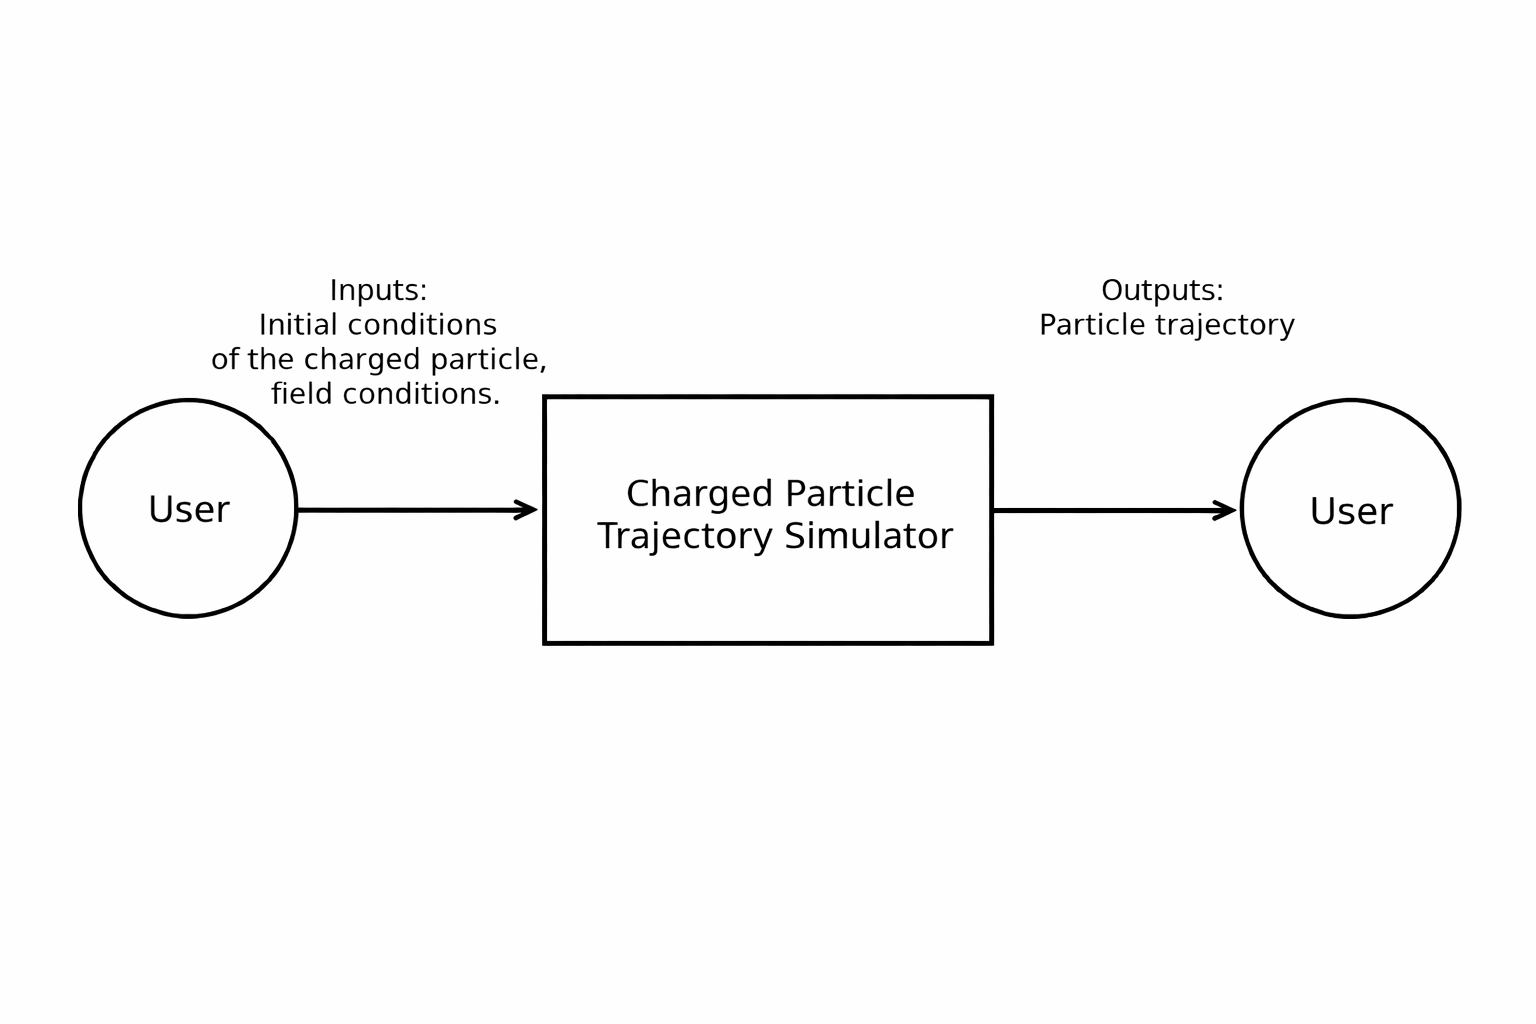
\includegraphics[width=\textwidth]{../../../../datafiles/trajecto/SystemContextFigure.png}
\caption{System Context}
\label{Figure:sysCtxDiag}
\end{center}
\end{figure}
The user provides the particle and field parameters; the software system computes and reports the particle trajectory:

\subsection{User Characteristics}
\label{Sec:UserChars}
The end user of Trajecto should have an understanding of undergraduate-level high school physics.

\subsection{System Constraints}
\label{Sec:SysConstraints}
There are no system constraints.

\section{Specific System Description}
\label{Sec:SpecSystDesc}
This section first presents the problem description, which gives a high-level view of the problem to be solved. This is followed by the solution characteristics specification, which presents the assumptions, theories, and definitions that are used.

\subsection{Problem Description}
\label{Sec:ProbDesc}
A system is needed to predict the trajectory of a charged particle moving through piecewise-uniform electric field and magnetic field regions.

\subsubsection{Terminology and Definitions}
\label{Sec:TermDefs}
This subsection provides a list of terms that are used in the subsequent sections and their meaning, with the purpose of reducing ambiguity and making it easier to correctly understand the requirements.

\begin{itemize}
\item{Charged particle: A particle that has a non-zero electric charge and can interact with electric and magnetic fields.}
\item{Electric field: A physical field that exerts an electric force on charged particles.}
\item{Magnetic field: A physical field that exerts a magnetic force on moving charged particles.}
\item{Lorentz force: The force on a charged particle due to electric and magnetic fields.}
\item{Trajectory: The path traced by a particle over time.}
\item{Field region: A spatial region in which the electric field and magnetic field are specified, typically treated as uniform within the region.}
\item{Detector line: A line at a specified location where the particle impact position is recorded.}
\item{Velocity selector: A configuration of crossed electric and magnetic fields that allows only particles with a particular velocity to pass through without deflection.}
\item{Cartesian coordinate system: A coordinate system that specifies each point uniquely in a plane by a set of numerical coordinates, which are the signed distances to the point from two fixed perpendicular oriented lines, measured in the same unit of length.}
\end{itemize}
\subsubsection{Physical System Description}
\label{Sec:PhysSyst}
The physical system of Trajecto, as shown in \hyperref[Figure:trajectoPhysSys]{Fig:trajectoPhysSys}, includes the following elements:

\begin{description}[font=\normalfont]
\item[PS1:]{A charged particle (the simulated particle)}
\item[PS2:]{The electric field in the particle's current region}
\item[PS3:]{The magnetic field perpendicular to the x-y plane}
\item[PS4:]{The detector line at a specified x-coordinate}
\end{description}
\begin{figure}[H]
\begin{center}
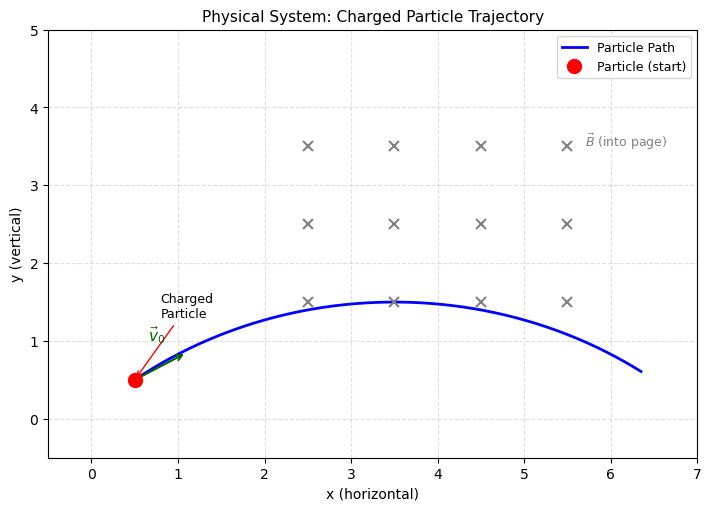
\includegraphics[width=0.6\textwidth]{../../../../datafiles/trajecto/trajecto.png}
\caption{The physical system description}
\label{Figure:trajectoPhysSys}
\end{center}
\end{figure}
\subsubsection{Goal Statements}
\label{Sec:GoalStmt}
Given the particle properties ($q$ and $m$), initial conditions (${x_{0}}$, ${y_{0}}$, ${v_{\text{x}0}}$, ${v_{\text{y}0}}$), the specification of electric and magnetic fields (${E_{\text{x}}}$, ${E_{\text{y}}}$, $B$), and detector geometry including ${t_{\text{final}}}$, the goal statements are:

\begin{description}[font=\normalfont]
\item[predictTrajectory:\phantomsection\label{predictTrajectory}]{Predict the trajectory of a charged particle under prescribed electric and magnetic fields.}
\item[determineDetectorOutcome:\phantomsection\label{determineDetectorOutcome}]{Determine impact position and time-of-flight at a specified detector line.}
\end{description}
\subsection{Solution Characteristics Specification}
\label{Sec:SolCharSpec}
The instance models that govern Trajecto are presented in the \hyperref[Sec:IMs]{Instance Model Section}. The information to understand the meaning of the instance models and their derivation is also presented, so that the instance models can be verified.

\subsubsection{Assumptions}
\label{Sec:Assumps}
This section simplifies the original problem and helps in developing the theoretical models by filling in the missing information for the physical system. The assumptions refine the scope by providing more detail.

\begin{description}[font=\normalfont]
\item[piecewiseUniform:\phantomsection\label{piecewiseUniform}]{The electric and magnetic fields are uniform within each field region and may change only at region boundaries.}
\item[singleParticle:\phantomsection\label{singleParticle}]{The particle is treated as a point mass and point charge. (RefBy: \hyperref[TM:lorentzForce]{TM:lorentzForce} and \hyperref[TM:eqnMotion]{TM:eqnMotion}.)}
\item[noInteractions:\phantomsection\label{noInteractions}]{Collisions and particle-particle interactions (including space-charge effects) are neglected.}
\item[prescribedFields:\phantomsection\label{prescribedFields}]{The electric and magnetic fields are user-specified and remain fixed during the simulation. (RefBy: \hyperref[TM:lorentzForce]{TM:lorentzForce}, \hyperref[TM:eqnMotion]{TM:eqnMotion}, and \hyperref[GD:xAccelEM]{GD:xAccelEM}.)}
\item[twoDMotion:\phantomsection\label{twoDMotion}]{The particle motion is confined to the x-y plane. (RefBy: \hyperref[GD:xAccelEM]{GD:xAccelEM} and \hyperref[lcExtendTo3D]{LC:lcExtendTo3D}.)}
\item[bPerpPlane:\phantomsection\label{bPerpPlane}]{The magnetic field is perpendicular to the x-y plane. (RefBy: \hyperref[GD:xAccelEM]{GD:xAccelEM}.)}
\item[eAxisAligned:\phantomsection\label{eAxisAligned}]{The electric field lies in the x-y plane and is aligned with a coordinate axis. (RefBy: \hyperref[GD:xAccelEM]{GD:xAccelEM}.)}
\item[rectRegions:\phantomsection\label{rectRegions}]{Field-region boundaries are rectangular and parallel to the x and y axes.}
\item[lineDetector:\phantomsection\label{lineDetector}]{The detector is modeled as a line located within the field region.}
\item[fullDetection:\phantomsection\label{fullDetection}]{The detector line is sufficiently long to record the impact point for any trajectory within the scope of the simulation.}
\item[lorentzOnly:\phantomsection\label{lorentzOnly}]{The particle dynamics are governed only by the Lorentz force; all other forces are neglected. (RefBy: \hyperref[TM:eqnMotion]{TM:eqnMotion} and \hyperref[ucLorentzForce]{UC:ucLorentzForce}.)}
\end{description}
\subsubsection{Theoretical Models}
\label{Sec:TMs}
This section focuses on the general equations and laws that Trajecto is based on.

\medskip
\noindent
\begin{minipage}{\textwidth}
\begin{tabular}{>{\raggedright}p{0.13\textwidth}>{\raggedright\arraybackslash}p{0.82\textwidth}}
\toprule \textbf{Refname} & \textbf{TM:velocity}
\phantomsection 
\label{TM:velocity}
\\ \midrule
Label & Velocity
        
\\ \midrule
Equation & \begin{displaymath}
           \resizeExpression{\symbf{v}\text{(}t\text{)}=\frac{\,d\symbf{p}\text{(}t\text{)}}{\,dt}}
           \end{displaymath}
\\ \midrule
Description & \begin{symbDescription}
              \item{$\symbf{v}\text{(}t\text{)}$ is the velocity ($\frac{\text{m}}{\text{s}}$)}
              \item{$t$ is the time (${\text{s}}$)}
              \item{$\symbf{p}\text{(}t\text{)}$ is the position (${\text{m}}$)}
              \end{symbDescription}
\\ \midrule
Source & \cite{velocityWiki}
         
\\ \midrule
RefBy & 
\\ \bottomrule
\end{tabular}
\end{minipage}

\medskip
\noindent
\begin{minipage}{\textwidth}
\begin{tabular}{>{\raggedright}p{0.13\textwidth}>{\raggedright\arraybackslash}p{0.82\textwidth}}
\toprule \textbf{Refname} & \textbf{TM:acceleration}
\phantomsection 
\label{TM:acceleration}
\\ \midrule
Label & Acceleration
        
\\ \midrule
Equation & \begin{displaymath}
           \resizeExpression{\symbf{a}\text{(}t\text{)}=\frac{\,d\symbf{v}\text{(}t\text{)}}{\,dt}}
           \end{displaymath}
\\ \midrule
Description & \begin{symbDescription}
              \item{$\symbf{a}\text{(}t\text{)}$ is the acceleration ($\frac{\text{m}}{\text{s}^{2}}$)}
              \item{$t$ is the time (${\text{s}}$)}
              \item{$\symbf{v}\text{(}t\text{)}$ is the velocity ($\frac{\text{m}}{\text{s}}$)}
              \end{symbDescription}
\\ \midrule
Source & \cite{accelerationWiki}
         
\\ \midrule
RefBy & 
\\ \bottomrule
\end{tabular}
\end{minipage}

\medskip
\noindent
\begin{minipage}{\textwidth}
\begin{tabular}{>{\raggedright}p{0.13\textwidth}>{\raggedright\arraybackslash}p{0.82\textwidth}}
\toprule \textbf{Refname} & \textbf{TM:lorentzForce}
\phantomsection 
\label{TM:lorentzForce}
\\ \midrule
Label & Lorentz force law
        
\\ \midrule
Equation & \begin{displaymath}
           \resizeExpression{\symbf{F}=q\,\left({E_{\text{x}}}+{v_{\text{y}}}\right)\,B}
           \end{displaymath}
\\ \midrule
Description & \begin{symbDescription}
              \item{$\symbf{F}$ is the force (${\text{N}}$)}
              \item{$q$ is the particle charge (${\text{C}}$)}
              \item{${E_{\text{x}}}$ is the x-component of the electric field ($\frac{\text{N}}{\text{C}}$)}
              \item{${v_{\text{y}}}$ is the y-velocity of the particle ($\frac{\text{m}}{\text{s}}$)}
              \item{$B$ is the out-of-plane magnetic flux density (${\text{T}}$)}
              \end{symbDescription}
\\ \midrule
Notes & The electromagnetic force on a charged particle is the sum of the electric force (q*E) and the magnetic force (q*(v x B)). For 2D planar motion with an out-of-plane magnetic field B, the x-component of the Lorentz force is Fx = q*(Ex + vy*B). Assumes \hyperref[singleParticle]{A:singleParticle}, \hyperref[prescribedFields]{A:prescribedFields}.
        
\\ \midrule
Source & --
         
\\ \midrule
RefBy & \hyperref[TM:eqnMotion]{TM:eqnMotion}
        
\\ \bottomrule
\end{tabular}
\end{minipage}

\medskip
\noindent
\begin{minipage}{\textwidth}
\begin{tabular}{>{\raggedright}p{0.13\textwidth}>{\raggedright\arraybackslash}p{0.82\textwidth}}
\toprule \textbf{Refname} & \textbf{TM:eqnMotion}
\phantomsection 
\label{TM:eqnMotion}
\\ \midrule
Label & Equation of motion under electromagnetic fields
        
\\ \midrule
Equation & \begin{displaymath}
           \resizeExpression{{a_{\text{x}}}=\frac{q}{m}\,\left({E_{\text{x}}}+{v_{\text{y}}}\right)\,B}
           \end{displaymath}
           \begin{displaymath}
           \resizeExpression{{a_{\text{y}}}=\frac{q}{m}\,\left({E_{\text{y}}}-{v_{\text{x}}}\right)\,B}
           \end{displaymath}
\\ \midrule
Description & \begin{symbDescription}
              \item{${a_{\text{x}}}$ is the x-acceleration of the particle ($\frac{\text{m}}{\text{s}^{2}}$)}
              \item{$q$ is the particle charge (${\text{C}}$)}
              \item{$m$ is the particle mass (${\text{kg}}$)}
              \item{${E_{\text{x}}}$ is the x-component of the electric field ($\frac{\text{N}}{\text{C}}$)}
              \item{${v_{\text{y}}}$ is the y-velocity of the particle ($\frac{\text{m}}{\text{s}}$)}
              \item{$B$ is the out-of-plane magnetic flux density (${\text{T}}$)}
              \end{symbDescription}
              \begin{symbDescription}
              \item{${a_{\text{y}}}$ is the y-acceleration of the particle ($\frac{\text{m}}{\text{s}^{2}}$)}
              \item{$q$ is the particle charge (${\text{C}}$)}
              \item{$m$ is the particle mass (${\text{kg}}$)}
              \item{${E_{\text{y}}}$ is the y-component of the electric field ($\frac{\text{N}}{\text{C}}$)}
              \item{${v_{\text{x}}}$ is the x-velocity of the particle ($\frac{\text{m}}{\text{s}}$)}
              \item{$B$ is the out-of-plane magnetic flux density (${\text{T}}$)}
              \end{symbDescription}
\\ \midrule
Notes & Combining Newton's second law with the Lorentz force law, (\hyperref[TM:lorentzForce]{TM:lorentzForce}), the equations of motion for each velocity component are obtained. The quantity q/m is the charge-to-mass ratio. Assumes \hyperref[singleParticle]{A:singleParticle}, \hyperref[prescribedFields]{A:prescribedFields}, \hyperref[lorentzOnly]{A:lorentzOnly}.
        
\\ \midrule
Source & --
         
\\ \midrule
RefBy & 
\\ \bottomrule
\end{tabular}
\end{minipage}

\subsubsection{General Definitions}
\label{Sec:GDs}
This section collects the laws and equations that will be used to build the instance models.

\medskip
\noindent
\begin{minipage}{\textwidth}
\begin{tabular}{>{\raggedright}p{0.13\textwidth}>{\raggedright\arraybackslash}p{0.82\textwidth}}
\toprule \textbf{Refname} & \textbf{GD:xAccelEM}
\phantomsection 
\label{GD:xAccelEM}
\\ \midrule
Label & X-acceleration under electromagnetic force
        
\\ \midrule
Units & $\frac{\text{m}}{\text{s}^{2}}$
        
\\ \midrule
Equation & \begin{displaymath}
           \resizeExpression{{a_{\text{x}}}=κ\,\left({E_{\text{x}}}+{v_{\text{y}}}\right)\,B}
           \end{displaymath}
\\ \midrule
Description & \begin{symbDescription}
              \item{${a_{\text{x}}}$ is the x-acceleration of the particle ($\frac{\text{m}}{\text{s}^{2}}$)}
              \item{$κ$ is the charge-to-mass ratio ($\frac{\text{C}}{\text{kg}}$)}
              \item{${E_{\text{x}}}$ is the x-component of the electric field ($\frac{\text{N}}{\text{C}}$)}
              \item{${v_{\text{y}}}$ is the y-velocity of the particle ($\frac{\text{m}}{\text{s}}$)}
              \item{$B$ is the out-of-plane magnetic flux density (${\text{T}}$)}
              \end{symbDescription}
\\ \midrule
Notes & Derived from the equation of motion by applying planar motion (\hyperref[twoDMotion]{A:twoDMotion}), out-of-plane B field (\hyperref[bPerpPlane]{A:bPerpPlane}), axis-aligned E field (\hyperref[eAxisAligned]{A:eAxisAligned}), and fixed fields (\hyperref[prescribedFields]{A:prescribedFields}). Here $κ$ = q/m is defined in \hyperref[DD:qOverm]{DD:qOverm}.
        
\\ \midrule
Source & --
         
\\ \midrule
RefBy & \hyperref[GD:yAccelEM]{GD:yAccelEM}
        
\\ \bottomrule
\end{tabular}
\end{minipage}

\medskip
\noindent
\begin{minipage}{\textwidth}
\begin{tabular}{>{\raggedright}p{0.13\textwidth}>{\raggedright\arraybackslash}p{0.82\textwidth}}
\toprule \textbf{Refname} & \textbf{GD:yAccelEM}
\phantomsection 
\label{GD:yAccelEM}
\\ \midrule
Label & Y-acceleration under electromagnetic force
        
\\ \midrule
Units & $\frac{\text{m}}{\text{s}^{2}}$
        
\\ \midrule
Equation & \begin{displaymath}
           \resizeExpression{{a_{\text{y}}}=κ\,\left({E_{\text{y}}}-{v_{\text{x}}}\right)\,B}
           \end{displaymath}
\\ \midrule
Description & \begin{symbDescription}
              \item{${a_{\text{y}}}$ is the y-acceleration of the particle ($\frac{\text{m}}{\text{s}^{2}}$)}
              \item{$κ$ is the charge-to-mass ratio ($\frac{\text{C}}{\text{kg}}$)}
              \item{${E_{\text{y}}}$ is the y-component of the electric field ($\frac{\text{N}}{\text{C}}$)}
              \item{${v_{\text{x}}}$ is the x-velocity of the particle ($\frac{\text{m}}{\text{s}}$)}
              \item{$B$ is the out-of-plane magnetic flux density (${\text{T}}$)}
              \end{symbDescription}
\\ \midrule
Notes & Derived from the equation of motion by applying the same 2D assumptions as for \hyperref[GD:xAccelEM]{GD:xAccelEM}.
        
\\ \midrule
Source & --
         
\\ \midrule
RefBy & 
\\ \bottomrule
\end{tabular}
\end{minipage}

\subsubsection{Data Definitions}
\label{Sec:DDs}
This section collects and defines all the data needed to build the instance models.

\medskip
\noindent
\begin{minipage}{\textwidth}
\begin{tabular}{>{\raggedright}p{0.13\textwidth}>{\raggedright\arraybackslash}p{0.82\textwidth}}
\toprule \textbf{Refname} & \textbf{DD:qOverm}
\phantomsection 
\label{DD:qOverm}
\\ \midrule
Label & Charge-to-mass ratio
        
\\ \midrule
Symbol & $κ$
         
\\ \midrule
Units & $\frac{\text{C}}{\text{kg}}$
        
\\ \midrule
Equation & \begin{displaymath}
           \resizeExpression{κ=\frac{q}{m}}
           \end{displaymath}
\\ \midrule
Description & \begin{symbDescription}
              \item{$κ$ is the charge-to-mass ratio ($\frac{\text{C}}{\text{kg}}$)}
              \item{$q$ is the particle charge (${\text{C}}$)}
              \item{$m$ is the particle mass (${\text{kg}}$)}
              \end{symbDescription}
\\ \midrule
Notes & The charge-to-mass ratio simplifies the equations of motion by combining the particle's charge $q$, and mass $m$ into a single parameter.
        
\\ \midrule
Source & --
         
\\ \midrule
RefBy & \hyperref[GD:xAccelEM]{GD:xAccelEM}
        
\\ \bottomrule
\end{tabular}
\end{minipage}

\subsubsection{Instance Models}
\label{Sec:IMs}
This section transforms the problem defined in the \hyperref[Sec:ProbDesc]{problem description} into one which is expressed in mathematical terms. It uses concrete symbols defined in the \hyperref[Sec:DDs]{data definitions} to replace the abstract symbols in the models identified in \hyperref[Sec:TMs]{theoretical models} and \hyperref[Sec:GDs]{general definitions}.

\medskip
\noindent
\begin{minipage}{\textwidth}
\begin{tabular}{>{\raggedright}p{0.13\textwidth}>{\raggedright\arraybackslash}p{0.82\textwidth}}
\toprule \textbf{Refname} & \textbf{IM:accelX}
\phantomsection 
\label{IM:accelX}
\\ \midrule
Label & X-component of acceleration
        
\\ \midrule
Input & $κ$, ${E_{\text{x}}}$, ${v_{\text{y}}}$, $B$
        
\\ \midrule
Output & ${a_{\text{x}}}$
         
\\ \midrule
Input Constraints & 
\\ \midrule
Output Constraints & 
\\ \midrule
Equation & \begin{displaymath}
           \resizeExpression{{a_{\text{x}}}=κ\,\left({E_{\text{x}}}+{v_{\text{y}}}\right)\,B}
           \end{displaymath}
\\ \midrule
Description & \begin{symbDescription}
              \item{${a_{\text{x}}}$ is the x-acceleration of the particle ($\frac{\text{m}}{\text{s}^{2}}$)}
              \item{$κ$ is the charge-to-mass ratio ($\frac{\text{C}}{\text{kg}}$)}
              \item{${E_{\text{x}}}$ is the x-component of the electric field ($\frac{\text{N}}{\text{C}}$)}
              \item{${v_{\text{y}}}$ is the y-velocity of the particle ($\frac{\text{m}}{\text{s}}$)}
              \item{$B$ is the out-of-plane magnetic flux density (${\text{T}}$)}
              \end{symbDescription}
\\ \midrule
Notes & This gives the acceleration of the particle in the x-direction due to the Lorentz force (see GD:xAccelEM).
        
\\ \midrule
Source & --
         
\\ \midrule
RefBy & 
\\ \bottomrule
\end{tabular}
\end{minipage}

\medskip
\noindent
\begin{minipage}{\textwidth}
\begin{tabular}{>{\raggedright}p{0.13\textwidth}>{\raggedright\arraybackslash}p{0.82\textwidth}}
\toprule \textbf{Refname} & \textbf{IM:accelY}
\phantomsection 
\label{IM:accelY}
\\ \midrule
Label & Y-component of acceleration
        
\\ \midrule
Input & $κ$, ${E_{\text{y}}}$, ${v_{\text{x}}}$, $B$
        
\\ \midrule
Output & ${a_{\text{y}}}$
         
\\ \midrule
Input Constraints & 
\\ \midrule
Output Constraints & 
\\ \midrule
Equation & \begin{displaymath}
           \resizeExpression{{a_{\text{y}}}=κ\,\left({E_{\text{y}}}-{v_{\text{x}}}\right)\,B}
           \end{displaymath}
\\ \midrule
Description & \begin{symbDescription}
              \item{${a_{\text{y}}}$ is the y-acceleration of the particle ($\frac{\text{m}}{\text{s}^{2}}$)}
              \item{$κ$ is the charge-to-mass ratio ($\frac{\text{C}}{\text{kg}}$)}
              \item{${E_{\text{y}}}$ is the y-component of the electric field ($\frac{\text{N}}{\text{C}}$)}
              \item{${v_{\text{x}}}$ is the x-velocity of the particle ($\frac{\text{m}}{\text{s}}$)}
              \item{$B$ is the out-of-plane magnetic flux density (${\text{T}}$)}
              \end{symbDescription}
\\ \midrule
Notes & This gives the acceleration of the particle in the y-direction due to the Lorentz force (see GD:yAccelEM).
        
\\ \midrule
Source & --
         
\\ \midrule
RefBy & 
\\ \bottomrule
\end{tabular}
\end{minipage}

\subsubsection{Data Constraints}
\label{Sec:DataConstraints}
The \hyperref[Table:InDataConstraints]{Input Data Constraints Table} shows the data constraints on the input variables. The column for physical constraints gives the physical limitations on the range of values that can be taken by the variable. The uncertainty column provides an estimate of the confidence with which the physical quantities can be measured. This information would be part of the input if one were performing an uncertainty quantification exercise. The constraints are conservative to give the user of the model the flexibility to experiment with unusual situations. The column of typical values is intended to provide a feel for a common scenario.

\begin{longtblr}
[caption={Input Data Constraints}]
{colspec={l l l l l}, rowhead=1, hline{1,Z}=\heavyrulewidth, hline{2}=\lightrulewidth}
\textbf{Var} & \textbf{Physical Constraints} & \textbf{Software Constraints} & \textbf{Typical Value} & \textbf{Uncert.}
\\
$B$ & -- & $-{B_{\text{max}}}\leq{}B\leq{}{B_{\text{max}}}$ & $0.01$ ${\text{T}}$ & 10.0$\%$
\\
${E_{\text{x}}}$ & -- & $-{E_{\text{max}}}\leq{}{E_{\text{x}}}\leq{}{E_{\text{max}}}$ & $0$ $\frac{\text{N}}{\text{C}}$ & 10.0$\%$
\\
${E_{\text{y}}}$ & -- & $-{E_{\text{max}}}\leq{}{E_{\text{y}}}\leq{}{E_{\text{max}}}$ & $1.0\cdot{}10^{3}$ $\frac{\text{N}}{\text{C}}$ & 10.0$\%$
\\
$m$ & $m\gt{}0$ & ${m_{\text{min}}}\leq{}m\leq{}{m_{\text{max}}}$ & $911.0\cdot{}10^{-33}$ ${\text{kg}}$ & 10.0$\%$
\\
$q$ & $q\gt{}0$ & $q\leq{}{q_{\text{max}}}$ & $160.0\cdot{}10^{-21}$ ${\text{C}}$ & 10.0$\%$
\\
${t_{\text{final}}}$ & ${t_{\text{final}}}\gt{}0$ & ${t_{\text{final}}}\leq{}{t_{\text{max}}}$ & $1.0\cdot{}10^{-6}$ ${\text{s}}$ & 0.0$\%$
\\
${v_{\text{x}0}}$ & -- & $-{v_{\text{max}}}\leq{}{v_{\text{x}0}}\leq{}{v_{\text{max}}}$ & $1.0\cdot{}10^{6}$ $\frac{\text{m}}{\text{s}}$ & 10.0$\%$
\\
${v_{\text{y}0}}$ & -- & $-{v_{\text{max}}}\leq{}{v_{\text{y}0}}\leq{}{v_{\text{max}}}$ & $0$ $\frac{\text{m}}{\text{s}}$ & 10.0$\%$
\\
${x_{0}}$ & -- & -- & $0$ ${\text{m}}$ & 0.0$\%$
\\
${y_{0}}$ & -- & -- & $0$ ${\text{m}}$ & 0.0$\%$
\label{Table:InDataConstraints}
\end{longtblr}
\subsubsection{Properties of a Correct Solution}
\label{Sec:CorSolProps}
There are no properties of a correct solution.

\section{Requirements}
\label{Sec:Requirements}
This section provides the functional requirements, the tasks and behaviours that the software is expected to complete, and the non-functional requirements, the qualities that the software is expected to exhibit.

\subsection{Functional Requirements}
\label{Sec:FRs}
This section provides the functional requirements, the tasks and behaviours that the software is expected to complete.

\begin{description}[font=\normalfont]
\item[Input-Values:\phantomsection\label{inputValues}]{Input the values from \hyperref[Table:ReqInputs]{Tab:ReqInputs}.}
\item[Echo-Inputs:\phantomsection\label{echoInputs}]{Echo the given inputs.}
\item[Compute-Trajectory:\phantomsection\label{computeTraj}]{Compute the trajectory of the charged particle using the equations of motion derived from the Lorentz force.}
\item[Report-Outputs:\phantomsection\label{reportOutputs}]{Report the final position, velocity, and whether the particle reaches the detector line.}
\end{description}
\begin{longtblr}
[caption={Required Inputs}]
{colspec={l l l}, rowhead=1, hline{1,Z}=\heavyrulewidth, hline{2}=\lightrulewidth}
\textbf{Symbol} & \textbf{Description} & \textbf{Units}
\\
$B$ & Out-of-plane magnetic flux density & ${\text{T}}$
\\
${E_{\text{x}}}$ & X-component of the electric field & $\frac{\text{N}}{\text{C}}$
\\
${E_{\text{y}}}$ & Y-component of the electric field & $\frac{\text{N}}{\text{C}}$
\\
$m$ & Particle mass & ${\text{kg}}$
\\
$q$ & Particle charge & ${\text{C}}$
\\
${t_{\text{final}}}$ & Final simulation time & ${\text{s}}$
\\
${v_{\text{x}0}}$ & Initial x-velocity & $\frac{\text{m}}{\text{s}}$
\\
${v_{\text{y}0}}$ & Initial y-velocity & $\frac{\text{m}}{\text{s}}$
\\
${x_{0}}$ & Initial x-position & ${\text{m}}$
\\
${y_{0}}$ & Initial y-position & ${\text{m}}$
\label{Table:ReqInputs}
\end{longtblr}
\subsection{Non-Functional Requirements}
\label{Sec:NFRs}
This section provides the non-functional requirements, the qualities that the software is expected to exhibit.

\begin{description}[font=\normalfont]
\item[Correctness:\phantomsection\label{correct}]{The outputs of the code have the \hyperref[Sec:CorSolProps]{properties of a correct solution}.}
\item[Maintainability:\phantomsection\label{maintainable}]{If a likely change is made to the finished software, it will take at most 10$\%$ of the original development time, assuming the same development resources are available.}
\item[Portability:\phantomsection\label{portable}]{The code shall be portable to multiple environments, particularly Windows, Mac OSX, and Linux.}
\end{description}
\section{Likely Changes}
\label{Sec:LCs}
This section lists the likely changes (LC) to be made to the software.

\begin{description}[font=\normalfont]
\item[lcExtendTo3D:\phantomsection\label{lcExtendTo3D}]{\hyperref[twoDMotion]{A:twoDMotion} - extend Trajecto to support three-dimensional (3D) motion, including a z-component of position, velocity, acceleration, electric field, and magnetic field.}
\end{description}
\section{Unlikely Changes}
\label{Sec:UCs}
This section lists the unlikely changes (UC) to be made to the software.

\begin{description}[font=\normalfont]
\item[ucLorentzForce:\phantomsection\label{ucLorentzForce}]{\hyperref[lorentzOnly]{A:lorentzOnly} - the Lorentz force law is a well-established physical principle and is unlikely to change.}
\end{description}
\section{Traceability Matrices and Graphs}
\label{Sec:TraceMatrices}
The purpose of the traceability matrices is to provide easy references on what has to be additionally modified if a certain component is changed. Every time a component is changed, the items in the column of that component that are marked with an ``X'' should be modified as well. \hyperref[Table:TraceMatAvsA]{Tab:TraceMatAvsA} shows the dependencies of the assumptions on each other. \hyperref[Table:TraceMatAvsAll]{Tab:TraceMatAvsAll} shows the dependencies of the data definitions, theoretical models, general definitions, instance models, requirements, likely changes, and unlikely changes on the assumptions. \hyperref[Table:TraceMatRefvsRef]{Tab:TraceMatRefvsRef} shows the dependencies of the data definitions, theoretical models, general definitions, and instance models on each other. \hyperref[Table:TraceMatAllvsR]{Tab:TraceMatAllvsR} shows the dependencies of the requirements and goal statements on the data definitions, theoretical models, general definitions, and instance models.

\begin{longtblr}
[caption={Traceability Matrix Showing the Connections Between Assumptions and Other Assumptions}]
{colspec={l l l l l l l l l l l l}, rowhead=1, hline{1,Z}=\heavyrulewidth, hline{2}=\lightrulewidth}
\textbf{} & \textbf{\hyperref[piecewiseUniform]{A:piecewiseUniform}} & \textbf{\hyperref[singleParticle]{A:singleParticle}} & \textbf{\hyperref[noInteractions]{A:noInteractions}} & \textbf{\hyperref[prescribedFields]{A:prescribedFields}} & \textbf{\hyperref[twoDMotion]{A:twoDMotion}} & \textbf{\hyperref[bPerpPlane]{A:bPerpPlane}} & \textbf{\hyperref[eAxisAligned]{A:eAxisAligned}} & \textbf{\hyperref[rectRegions]{A:rectRegions}} & \textbf{\hyperref[lineDetector]{A:lineDetector}} & \textbf{\hyperref[fullDetection]{A:fullDetection}} & \textbf{\hyperref[lorentzOnly]{A:lorentzOnly}}
\\
\hyperref[piecewiseUniform]{A:piecewiseUniform} &  &  &  &  &  &  &  &  &  &  & 
\\
\hyperref[singleParticle]{A:singleParticle} &  &  &  &  &  &  &  &  &  &  & 
\\
\hyperref[noInteractions]{A:noInteractions} &  &  &  &  &  &  &  &  &  &  & 
\\
\hyperref[prescribedFields]{A:prescribedFields} &  &  &  &  &  &  &  &  &  &  & 
\\
\hyperref[twoDMotion]{A:twoDMotion} &  &  &  &  &  &  &  &  &  &  & 
\\
\hyperref[bPerpPlane]{A:bPerpPlane} &  &  &  &  &  &  &  &  &  &  & 
\\
\hyperref[eAxisAligned]{A:eAxisAligned} &  &  &  &  &  &  &  &  &  &  & 
\\
\hyperref[rectRegions]{A:rectRegions} &  &  &  &  &  &  &  &  &  &  & 
\\
\hyperref[lineDetector]{A:lineDetector} &  &  &  &  &  &  &  &  &  &  & 
\\
\hyperref[fullDetection]{A:fullDetection} &  &  &  &  &  &  &  &  &  &  & 
\\
\hyperref[lorentzOnly]{A:lorentzOnly} &  &  &  &  &  &  &  &  &  &  & 
\label{Table:TraceMatAvsA}
\end{longtblr}
\begin{longtblr}
[caption={Traceability Matrix Showing the Connections Between Assumptions and Other Items}]
{colspec={l l l l l l l l l l l l}, rowhead=1, hline{1,Z}=\heavyrulewidth, hline{2}=\lightrulewidth}
\textbf{} & \textbf{\hyperref[piecewiseUniform]{A:piecewiseUniform}} & \textbf{\hyperref[singleParticle]{A:singleParticle}} & \textbf{\hyperref[noInteractions]{A:noInteractions}} & \textbf{\hyperref[prescribedFields]{A:prescribedFields}} & \textbf{\hyperref[twoDMotion]{A:twoDMotion}} & \textbf{\hyperref[bPerpPlane]{A:bPerpPlane}} & \textbf{\hyperref[eAxisAligned]{A:eAxisAligned}} & \textbf{\hyperref[rectRegions]{A:rectRegions}} & \textbf{\hyperref[lineDetector]{A:lineDetector}} & \textbf{\hyperref[fullDetection]{A:fullDetection}} & \textbf{\hyperref[lorentzOnly]{A:lorentzOnly}}
\\
\hyperref[DD:qOverm]{DD:qOverm} &  &  &  &  &  &  &  &  &  &  & 
\\
\hyperref[TM:velocity]{TM:velocity} &  &  &  &  &  &  &  &  &  &  & 
\\
\hyperref[TM:acceleration]{TM:acceleration} &  &  &  &  &  &  &  &  &  &  & 
\\
\hyperref[TM:lorentzForce]{TM:lorentzForce} &  & X &  & X &  &  &  &  &  &  & 
\\
\hyperref[TM:eqnMotion]{TM:eqnMotion} &  & X &  & X &  &  &  &  &  &  & X
\\
\hyperref[GD:xAccelEM]{GD:xAccelEM} &  &  &  & X & X & X & X &  &  &  & 
\\
\hyperref[GD:yAccelEM]{GD:yAccelEM} &  &  &  &  &  &  &  &  &  &  & 
\\
\hyperref[IM:accelX]{IM:accelX} &  &  &  &  &  &  &  &  &  &  & 
\\
\hyperref[IM:accelY]{IM:accelY} &  &  &  &  &  &  &  &  &  &  & 
\\
\hyperref[inputValues]{FR:Input-Values} &  &  &  &  &  &  &  &  &  &  & 
\\
\hyperref[echoInputs]{FR:Echo-Inputs} &  &  &  &  &  &  &  &  &  &  & 
\\
\hyperref[computeTraj]{FR:Compute-Trajectory} &  &  &  &  &  &  &  &  &  &  & 
\\
\hyperref[reportOutputs]{FR:Report-Outputs} &  &  &  &  &  &  &  &  &  &  & 
\\
\hyperref[correct]{NFR:Correctness} &  &  &  &  &  &  &  &  &  &  & 
\\
\hyperref[maintainable]{NFR:Maintainability} &  &  &  &  &  &  &  &  &  &  & 
\\
\hyperref[portable]{NFR:Portability} &  &  &  &  &  &  &  &  &  &  & 
\\
\hyperref[lcExtendTo3D]{LC:lcExtendTo3D} &  &  &  &  & X &  &  &  &  &  & 
\\
\hyperref[ucLorentzForce]{UC:ucLorentzForce} &  &  &  &  &  &  &  &  &  &  & X
\label{Table:TraceMatAvsAll}
\end{longtblr}
\begin{longtblr}
[caption={Traceability Matrix Showing the Connections Between Items and Other Sections}]
{colspec={l l l l l l l l l l}, rowhead=1, hline{1,Z}=\heavyrulewidth, hline{2}=\lightrulewidth}
\textbf{} & \textbf{\hyperref[DD:qOverm]{DD:qOverm}} & \textbf{\hyperref[TM:velocity]{TM:velocity}} & \textbf{\hyperref[TM:acceleration]{TM:acceleration}} & \textbf{\hyperref[TM:lorentzForce]{TM:lorentzForce}} & \textbf{\hyperref[TM:eqnMotion]{TM:eqnMotion}} & \textbf{\hyperref[GD:xAccelEM]{GD:xAccelEM}} & \textbf{\hyperref[GD:yAccelEM]{GD:yAccelEM}} & \textbf{\hyperref[IM:accelX]{IM:accelX}} & \textbf{\hyperref[IM:accelY]{IM:accelY}}
\\
\hyperref[DD:qOverm]{DD:qOverm} &  &  &  &  &  &  &  &  & 
\\
\hyperref[TM:velocity]{TM:velocity} &  &  &  &  &  &  &  &  & 
\\
\hyperref[TM:acceleration]{TM:acceleration} &  &  &  &  &  &  &  &  & 
\\
\hyperref[TM:lorentzForce]{TM:lorentzForce} &  &  &  &  &  &  &  &  & 
\\
\hyperref[TM:eqnMotion]{TM:eqnMotion} &  &  &  & X &  &  &  &  & 
\\
\hyperref[GD:xAccelEM]{GD:xAccelEM} & X &  &  &  &  &  &  &  & 
\\
\hyperref[GD:yAccelEM]{GD:yAccelEM} &  &  &  &  &  & X &  &  & 
\\
\hyperref[IM:accelX]{IM:accelX} &  &  &  &  &  &  &  &  & 
\\
\hyperref[IM:accelY]{IM:accelY} &  &  &  &  &  &  &  &  & 
\label{Table:TraceMatRefvsRef}
\end{longtblr}
\begin{longtblr}
[caption={Traceability Matrix Showing the Connections Between Requirements, Goal Statements and Other Items}]
{colspec={l l l l l l l l l l l l l l l l l}, rowhead=1, hline{1,Z}=\heavyrulewidth, hline{2}=\lightrulewidth}
\textbf{} & \textbf{\hyperref[DD:qOverm]{DD:qOverm}} & \textbf{\hyperref[TM:velocity]{TM:velocity}} & \textbf{\hyperref[TM:acceleration]{TM:acceleration}} & \textbf{\hyperref[TM:lorentzForce]{TM:lorentzForce}} & \textbf{\hyperref[TM:eqnMotion]{TM:eqnMotion}} & \textbf{\hyperref[GD:xAccelEM]{GD:xAccelEM}} & \textbf{\hyperref[GD:yAccelEM]{GD:yAccelEM}} & \textbf{\hyperref[IM:accelX]{IM:accelX}} & \textbf{\hyperref[IM:accelY]{IM:accelY}} & \textbf{\hyperref[inputValues]{FR:Input-Values}} & \textbf{\hyperref[echoInputs]{FR:Echo-Inputs}} & \textbf{\hyperref[computeTraj]{FR:Compute-Trajectory}} & \textbf{\hyperref[reportOutputs]{FR:Report-Outputs}} & \textbf{\hyperref[correct]{NFR:Correctness}} & \textbf{\hyperref[maintainable]{NFR:Maintainability}} & \textbf{\hyperref[portable]{NFR:Portability}}
\\
\hyperref[predictTrajectory]{GS:predictTrajectory} &  &  &  &  &  &  &  &  &  &  &  &  &  &  &  & 
\\
\hyperref[determineDetectorOutcome]{GS:determineDetectorOutcome} &  &  &  &  &  &  &  &  &  &  &  &  &  &  &  & 
\\
\hyperref[inputValues]{FR:Input-Values} &  &  &  &  &  &  &  &  &  &  &  &  &  &  &  & 
\\
\hyperref[echoInputs]{FR:Echo-Inputs} &  &  &  &  &  &  &  &  &  &  &  &  &  &  &  & 
\\
\hyperref[computeTraj]{FR:Compute-Trajectory} &  &  &  &  &  &  &  &  &  &  &  &  &  &  &  & 
\\
\hyperref[reportOutputs]{FR:Report-Outputs} &  &  &  &  &  &  &  &  &  &  &  &  &  &  &  & 
\\
\hyperref[correct]{NFR:Correctness} &  &  &  &  &  &  &  &  &  &  &  &  &  &  &  & 
\\
\hyperref[maintainable]{NFR:Maintainability} &  &  &  &  &  &  &  &  &  &  &  &  &  &  &  & 
\\
\hyperref[portable]{NFR:Portability} &  &  &  &  &  &  &  &  &  &  &  &  &  &  &  & 
\label{Table:TraceMatAllvsR}
\end{longtblr}
The purpose of the traceability graphs is also to provide easy references on what has to be additionally modified if a certain component is changed. The arrows in the graphs represent dependencies. The component at the tail of an arrow is depended on by the component at the head of that arrow. Therefore, if a component is changed, the components that it points to should also be changed. \hyperref[Figure:TraceGraphAvsA]{Fig:TraceGraphAvsA} shows the dependencies of assumptions on each other. \hyperref[Figure:TraceGraphAvsAll]{Fig:TraceGraphAvsAll} shows the dependencies of data definitions, theoretical models, general definitions, instance models, requirements, likely changes, and unlikely changes on the assumptions. \hyperref[Figure:TraceGraphRefvsRef]{Fig:TraceGraphRefvsRef} shows the dependencies of data definitions, theoretical models, general definitions, and instance models on each other. \hyperref[Figure:TraceGraphAllvsR]{Fig:TraceGraphAllvsR} shows the dependencies of requirements and goal statements on the data definitions, theoretical models, general definitions, and instance models. \hyperref[Figure:TraceGraphAllvsAll]{Fig:TraceGraphAllvsAll} shows the dependencies of dependencies of assumptions, models, definitions, requirements, goals, and changes with each other.

\begin{figure}[H]
\begin{center}
\includesvg[width=\textwidth, inkscapelatex = false]{../../../../traceygraphs/trajecto/avsa}
\caption{TraceGraphAvsA}
\label{Figure:TraceGraphAvsA}
\end{center}
\end{figure}
\begin{figure}[H]
\begin{center}
\includesvg[width=\textwidth, inkscapelatex = false]{../../../../traceygraphs/trajecto/avsall}
\caption{TraceGraphAvsAll}
\label{Figure:TraceGraphAvsAll}
\end{center}
\end{figure}
\begin{figure}[H]
\begin{center}
\includesvg[width=\textwidth, inkscapelatex = false]{../../../../traceygraphs/trajecto/refvsref}
\caption{TraceGraphRefvsRef}
\label{Figure:TraceGraphRefvsRef}
\end{center}
\end{figure}
\begin{figure}[H]
\begin{center}
\includesvg[width=\textwidth, inkscapelatex = false]{../../../../traceygraphs/trajecto/allvsr}
\caption{TraceGraphAllvsR}
\label{Figure:TraceGraphAllvsR}
\end{center}
\end{figure}
\begin{figure}[H]
\begin{center}
\includesvg[width=\textwidth, inkscapelatex = false]{../../../../traceygraphs/trajecto/allvsall}
\caption{TraceGraphAllvsAll}
\label{Figure:TraceGraphAllvsAll}
\end{center}
\end{figure}
For convenience, the following graphs can be found at the links below:

\begin{itemize}
\item{\hyperref{../../../../traceygraphs/trajecto/avsa.svg}{}{}{TraceGraphAvsA}}
\item{\hyperref{../../../../traceygraphs/trajecto/avsall.svg}{}{}{TraceGraphAvsAll}}
\item{\hyperref{../../../../traceygraphs/trajecto/refvsref.svg}{}{}{TraceGraphRefvsRef}}
\item{\hyperref{../../../../traceygraphs/trajecto/allvsr.svg}{}{}{TraceGraphAllvsR}}
\item{\hyperref{../../../../traceygraphs/trajecto/allvsall.svg}{}{}{TraceGraphAllvsAll}}
\end{itemize}
\section{Values of Auxiliary Constants}
\label{Sec:AuxConstants}
There are no auxiliary constants.

\section{References}
\label{Sec:References}
\begin{filecontents*}{bibfile.bib}
@mastersthesis{koothoor2013,
author={Koothoor, Nirmitha},
title={A Document Driven Approach to Certifying Scientific Computing Software},
school={McMaster University},
year={2013},
address={Hamilton, ON, Canada}}
@article{parnasClements1986,
author={Parnas, David L. and Clements, P. C.},
title={A rational design process: How and why to fake it},
journal={IEEE Transactions on Software Engineering},
year={1986},
month=feb,
volume={12},
number={2},
pages={251--257},
address={Washington, USA}}
@article{smithKoothoor2016,
author={Smith, W. Spencer and Koothoor, Nirmitha},
title={A Document-Driven Method for Certifying Scientific Computing Software for Use in Nuclear Safety Analysis},
journal={Nuclear Engineering and Technology},
year={2016},
month=apr,
volume={48},
number={2},
pages={404--418},
howpublished={\url{http://www.sciencedirect.com/science/article/pii/S1738573315002582}}}
@inproceedings{smithLai2005,
author={Smith, W. Spencer and Lai, Lei},
title={A new requirements template for scientific computing},
booktitle={Proceedings of the First International Workshop on Situational Requirements Engineering Processes - Methods, Techniques and Tools to Support Situation-Specific Requirements Engineering Processes, SREP'05},
year={2005},
editor={Agerfalk, PJ and Kraiem, N. and Ralyte, J.},
address={Paris, France},
pages={107--121},
note={In conjunction with 13th IEEE International Requirements Engineering Conference,}}
@article{smithEtAl2007,
author={Smith, W. Spencer and Lai, Lei and Khedri, Ridha},
title={Requirements Analysis for Engineering Computation: A Systematic Approach for Improving Software Reliability},
journal={Reliable Computing, Special Issue on Reliable Engineering Computation},
year={2007},
month=feb,
volume={13},
number={1},
pages={83--107},
howpublished={\url{https://doi.org/10.1007/s11155-006-9020-7}}}
@misc{accelerationWiki,
author={Wikipedia Contributors},
title={Acceleration},
howpublished={\url{https://en.wikipedia.org/wiki/Acceleration}},
month=jun,
year={2019}}
@misc{velocityWiki,
author={Wikipedia Contributors},
title={Velocity},
howpublished={\url{https://en.wikipedia.org/wiki/Velocity}},
month=jun,
year={2019}}
\end{filecontents*}
\nocite{*}
\bibstyle{ieeetr}
\printbibliography[heading=none]
\end{document}
